\documentclass{beamer}
\setbeamertemplate{navigation symbols}{}
%\usefonttheme[onlymath]{serif}
\usepackage{beamerthemeshadow}
\usepackage[utf8]{inputenc}
\usepackage{amsmath}
\usepackage{amsfonts}
\usepackage{amssymb}
\usepackage[french]{babel}
\usetheme{Antibes}
\usecolortheme[RGB={15,110,40}]{structure}

\begin{document}


\title{Pilotage automatique d'un voilier}  
\author{Cabrillana Jean-Manuel}
\date{\today} 

\begin{frame}
\titlepage
\end{frame}

\begin{frame}
\frametitle{Plan}
\textbf{Problématique:} Comment piloter un voilier de façon optimale?
\tableofcontents
\end{frame} 


\section{Calcul d'une route de navigation}
 
\subsection{Polaire des vitesses}

\begin{frame}
\begin{figure}
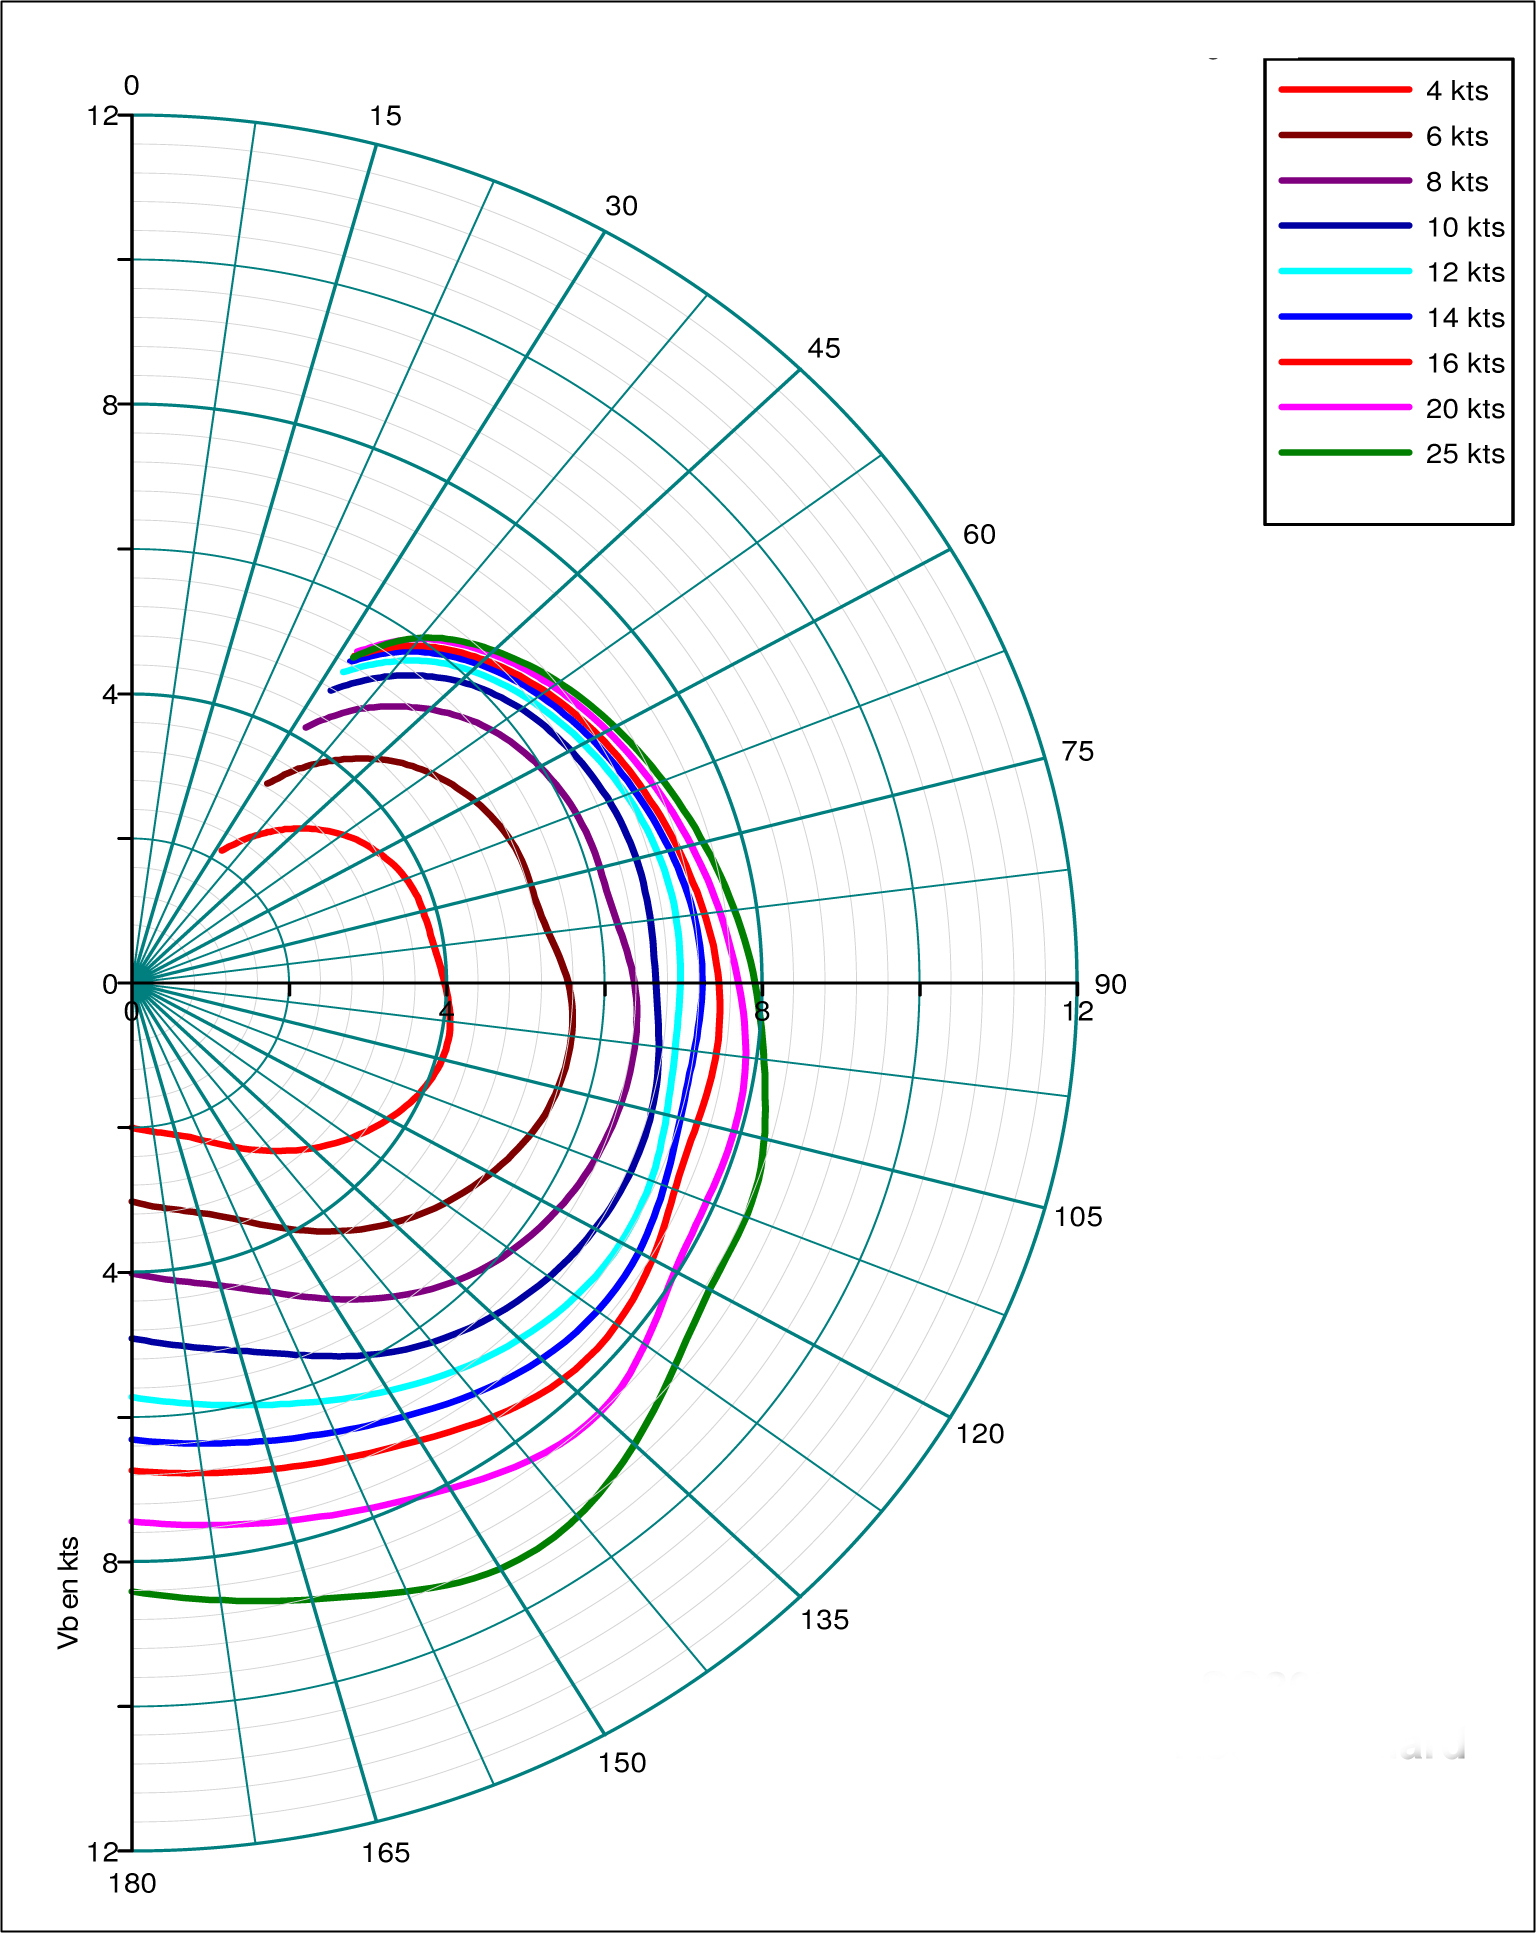
\includegraphics[scale=0.4]{polaire.jpg} 
\caption{Vitesse du voilier en fonction de l'angle avec le vent et de sa vitesse}
\end{figure}
\end{frame}


\subsection{Données météorologiques (fichier GRIB)}

\begin{frame}\frametitle{représentation cartographique} 
\begin{figure}
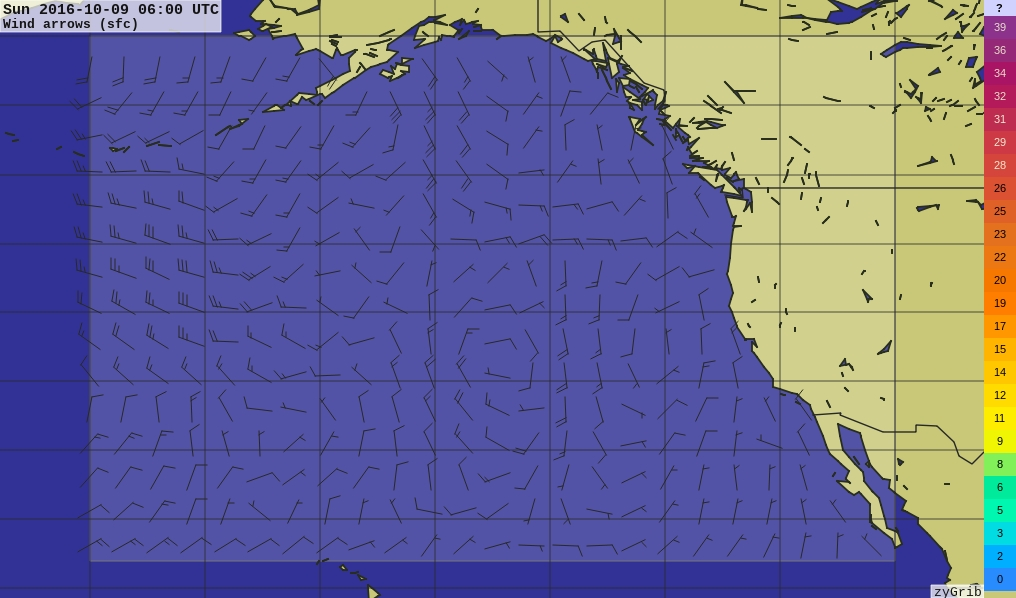
\includegraphics[scale=0.4]{grille1.jpg} 
\caption{Golfe d'Alaska - Océan Pacifique}
\end{figure}
\end{frame}

\begin{frame}\frametitle{représentation cartographique} 
\begin{figure}
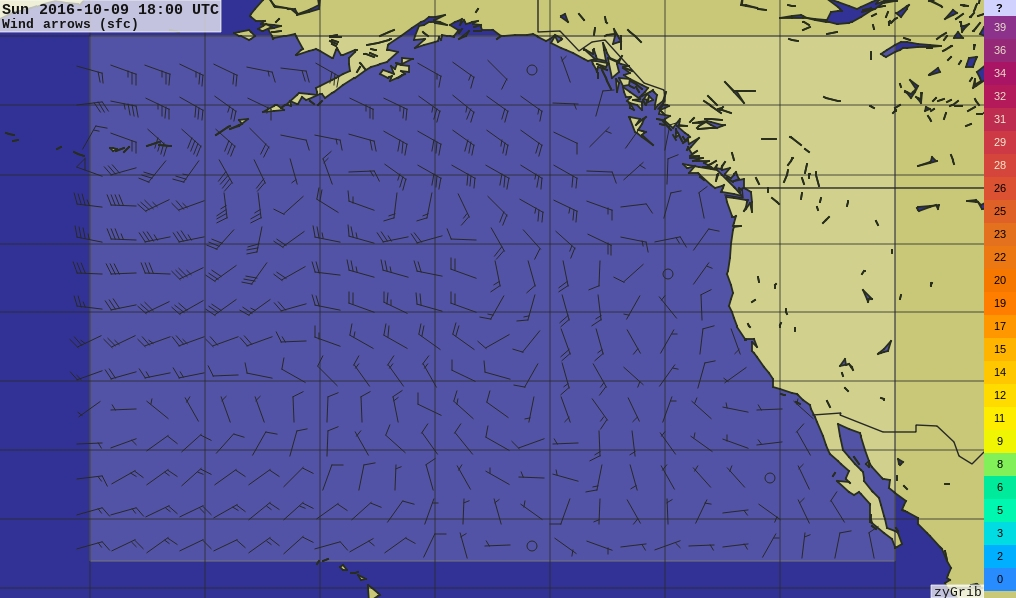
\includegraphics[scale=0.4]{grille2.jpg} 
\end{figure}
\end{frame}

\begin{frame}\frametitle{représentation cartographique} 
\begin{figure}
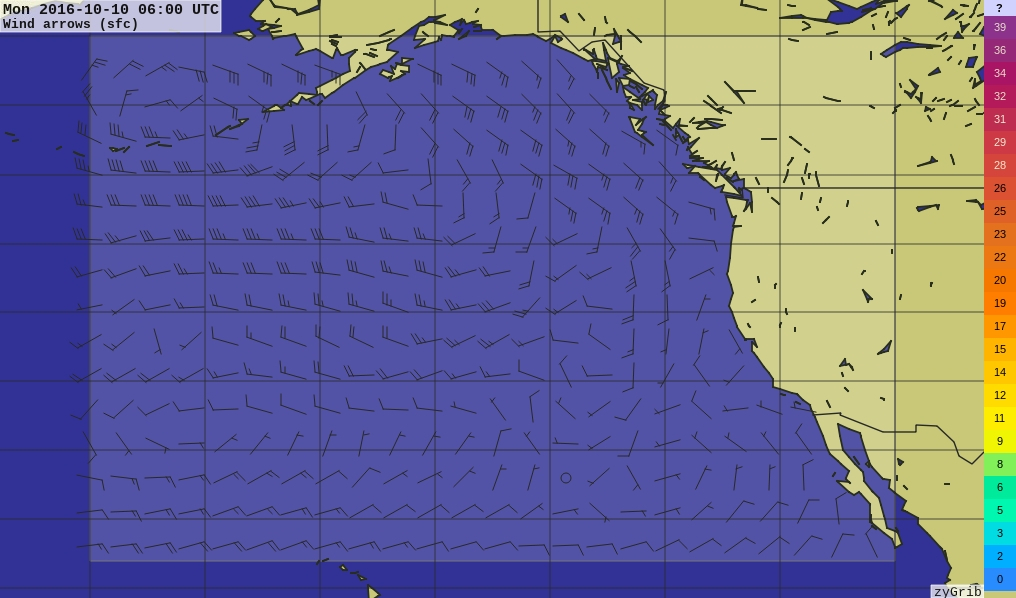
\includegraphics[scale=0.4]{grille3.jpg} 
\end{figure}
\end{frame}

\begin{frame}\frametitle{représentation cartographique} 
\begin{figure}
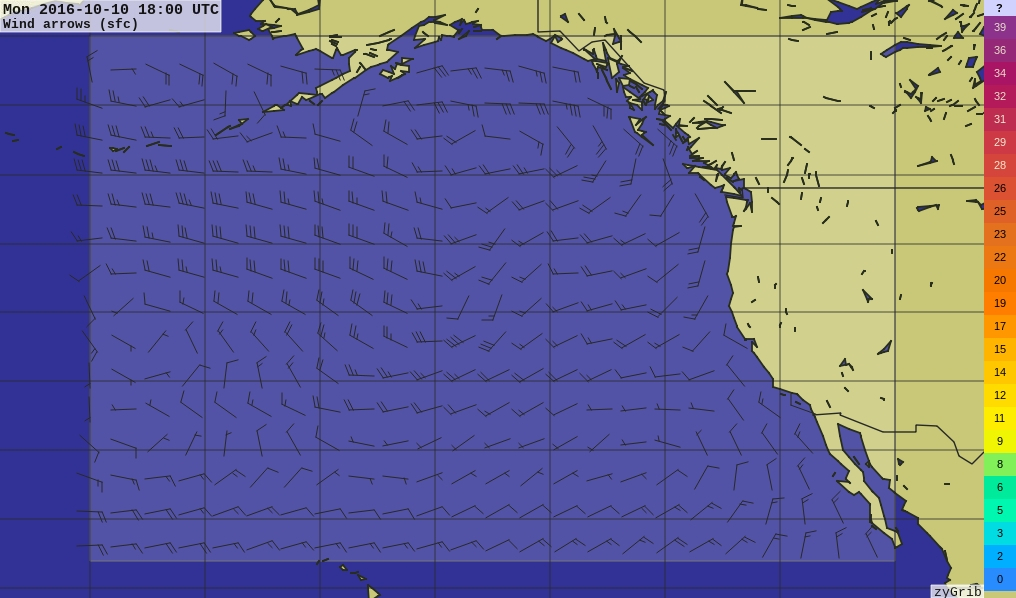
\includegraphics[scale=0.4]{grille4.jpg} 
\end{figure}
\end{frame}


\subsection{Algorithme de Dijkstra}

\begin{frame}\frametitle{Structure de données}
\begin{columns}

	\begin{column}{5cm}
	Structures utilisées:
	\begin{itemize}
	\item Un graphe G = (S, A)
	\item Les sommets de S sont des triplets (x,y,t) (aussi associés a un booléen "marqué" et un coût en temps)
	\item Une liste triée selon le coût au sommet de départ des voisins du sous-graphe (V)
	\end{itemize}
	\end{column}
	
	\begin{column}{5cm}
	\begin{figure}
	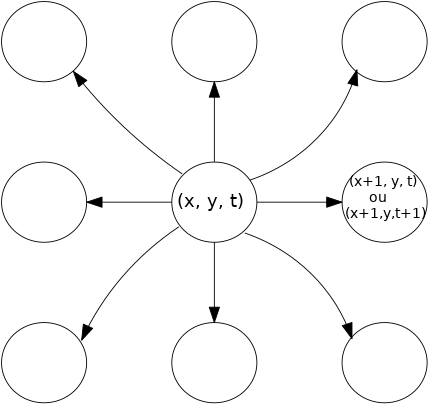
\includegraphics[scale=0.3]{graphe.png} 
	\caption{Exemple de sommets}
	\end{figure}
	\end{column}
	
\end{columns}
\end{frame}



\begin{frame}\frametitle{Algorithme}
	\begin{block}{Objectif}
	Construire un sous-graphe P, initialement vide, pour lequel les coût au sommet de départ sont minimaux; renvoyer le chemin 	trouvé.
	\end{block}
	\begin{exampleblock}{Algorithme}
	Tant qu'il existe un sommet dans V:
	\begin{description}
	\item Choisir un sommet a dans V de plus petit coût
	\item Mettre a dans P 
	\item Pour chaque sommet v hors de  P voisin de a:
	\item    -\;  v.cout = min($v$.cout, $a$.cout + $p(a,v)$)
	\item    -\;  Ajouter v à V si besoin
	\item Fin pour et Fin Tant que
	\\Retracer le chemin\\
	\end{description}
	\end{exampleblock}
\end{frame}


\begin{frame}\frametitle{Algorithme}
\begin{block}{Complexité}
La seule opération qui n'est pas à temps constant est la suppression et l'insertion dans V qui sont en temps logarithmique par rapport à sa taille, qui est au maximum de $N$. A chaque itération de l'algorithme, un sommet est traité. Donc il y a au plus $N$ itérations. La complexité est en $\Theta( Nlog(N))$
\end{block}
\end{frame}

\begin{frame}\frametitle{résultats}
\begin{figure}
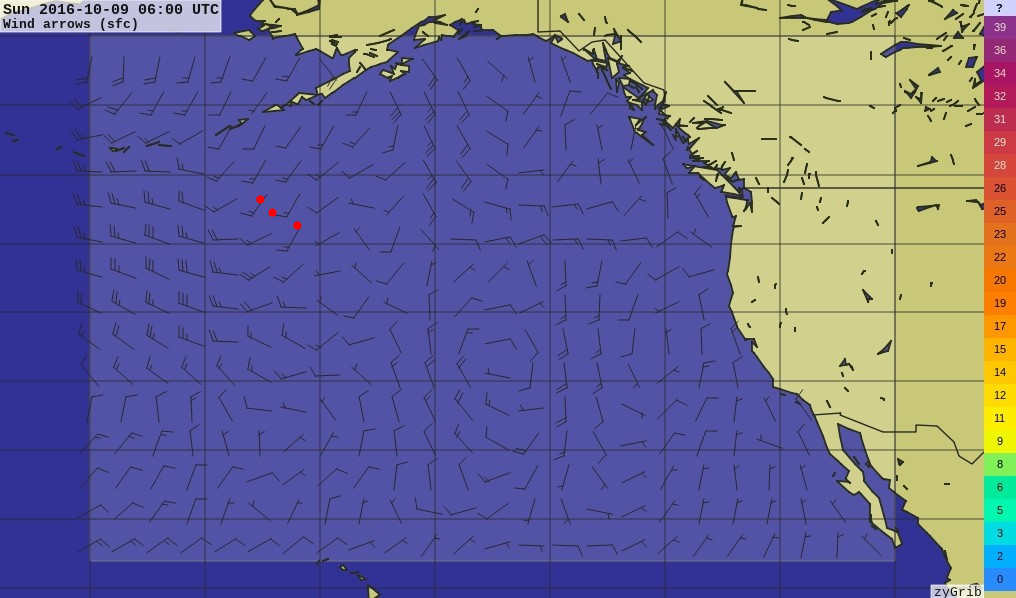
\includegraphics[scale=0.3]{result11.jpg} 
\end{figure}
\end{frame}

\begin{frame}\frametitle{résultats}
\begin{figure}
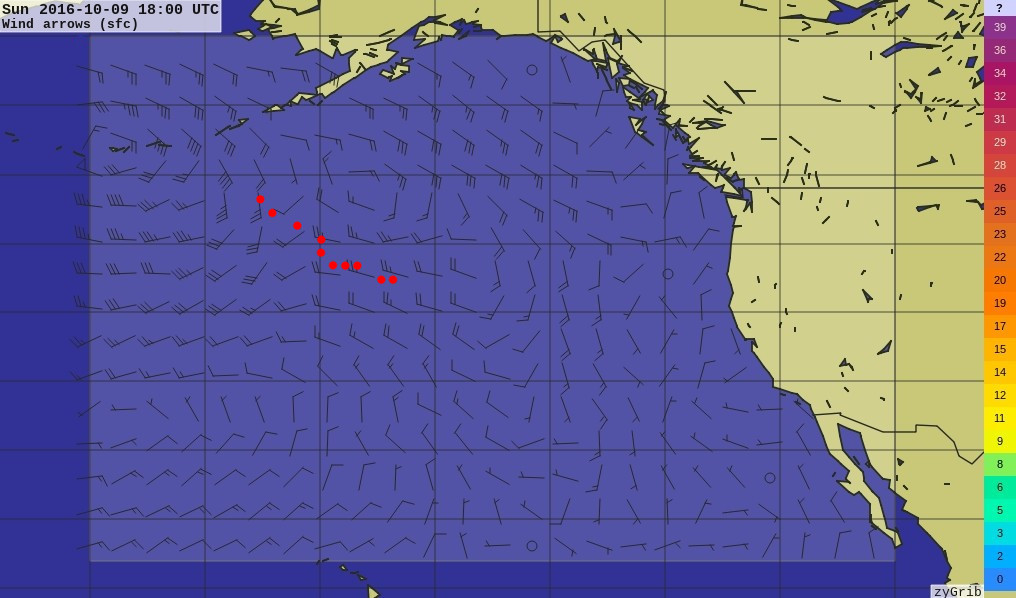
\includegraphics[scale=0.3]{result22.jpg} 
\end{figure}
\end{frame}

\begin{frame}\frametitle{résultats}
\begin{figure}
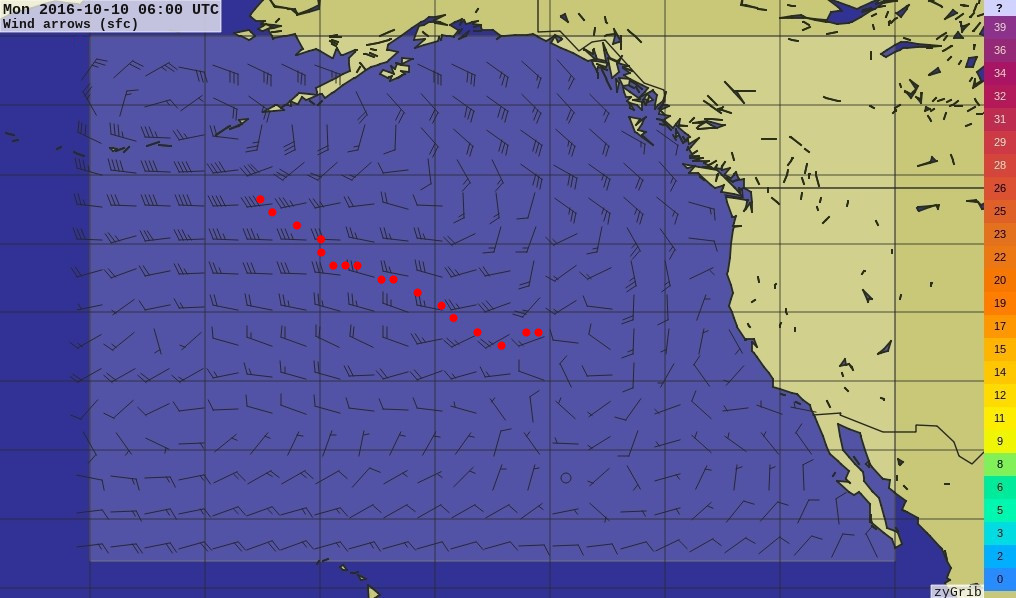
\includegraphics[scale=0.3]{result33.jpg} 
\end{figure}
\end{frame}

\begin{frame}\frametitle{résultats}
\begin{figure}
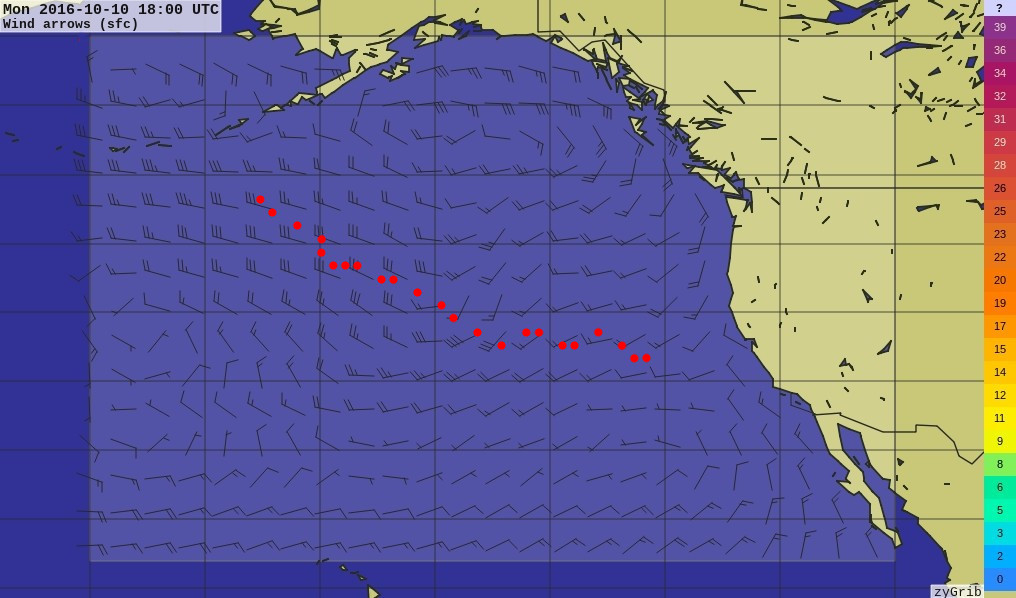
\includegraphics[scale=0.3]{result44.jpg} 
\end{figure}
\end{frame}


\section{Simulation du voilier}

\subsection{Le vent en mer}

\begin{frame}\frametitle{II Simulation du voilier: du vent}
\begin{figure}
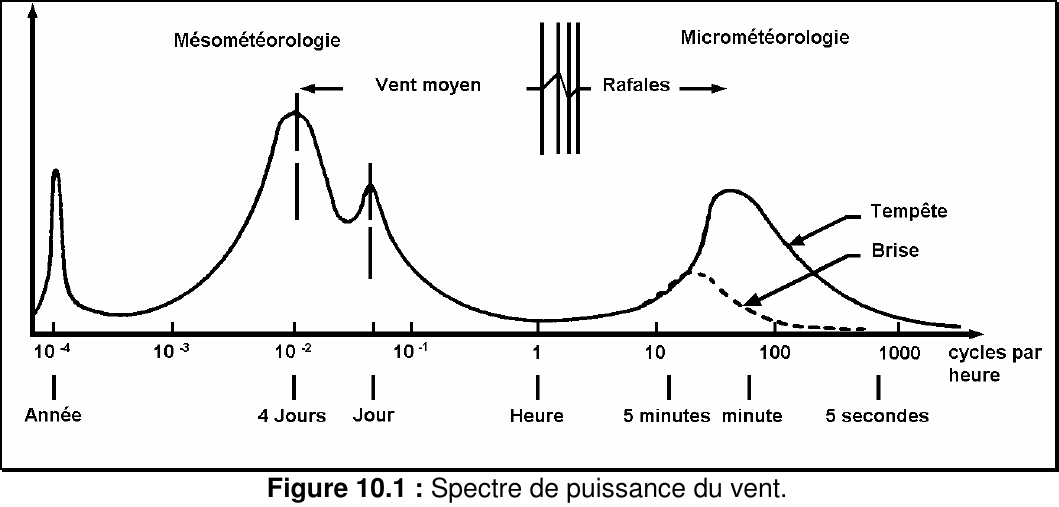
\includegraphics[scale=0.26]{spectre_vent.jpg} 
\end{figure}
\textbf{ Forme discrétisée:}
\\
\[ w(t) = \sum_{i=1}^{n} a_{i}cos(2\pi f_{i} + \phi_{i}) \]
\end{frame}

\begin{frame}\frametitle{Effort sur la voile}
Norme de la force:
\[ F_{v} = \frac{1}{2}\rho S V^{2} C(\alpha) \]
Avec:
\begin{itemize}
\item $\rho$ la masse volumique du fluide (l'air)
\item $S$ la surface de référence
\item $V$ la vitesse du vent
\item $C$ le coefficient aérodynamique
\item $\alpha$ l'angle d'incidence avec le vent
\end{itemize}
\end{frame}

\begin{frame}[plain]
\begin{figure}
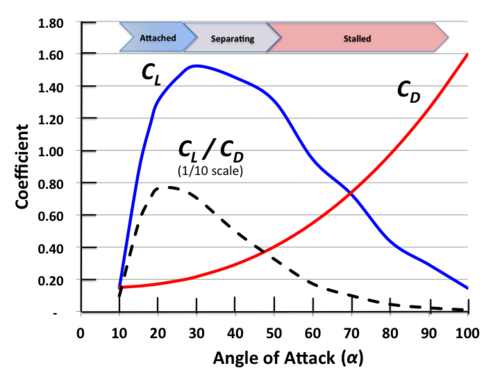
\includegraphics[scale=0.45]{LDcoefficients.png} 
\caption{Coefficients de traînée et de portance de la voile}
La voile est réglée au maximum de $C_{L}/C_{D}$ Pour avoir le meilleur maintien de cap possible.
\end{figure}
\end{frame}

\subsection{Forces hydrodynamiques}

\begin{frame}[plain]
\begin{itemize}
\item Forces de trainé et de portance:
\[ F = \frac{1}{2}\rho S V^{2} C \]
\item Force due aux vagues (force significative pour une vitesse de vent supérieure à 22 noeuds):
\[ F = K(\gamma)cos(wt - \vec{k} \centerdot \vec{OM} + \phi) \]

\end{itemize}
\begin{figure}
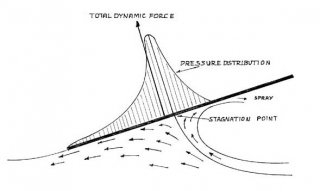
\includegraphics[scale=0.7]{planing.jpg} 
\end{figure}
\end{frame}

\subsection{Dynamique du voilier}

\begin{frame}\frametitle{dynamique du voilier}
\begin{columns}
\begin{column}{5cm}
Théorème de la résultante cinétique au voilier:
\[ m \vec{a} = \sum \vec{F} \]
Théorème du moment cinétique selon l'axe (Gz):
\[ J \frac{d \omega}{dt} = \sum M \]
Equation de récurrence:
\[ \vec{v_{i+1}} = \vec{v_{i}} + \frac{\sum \vec{F_{i}}}{m}dt \]
\end{column}
\begin{column}{5cm}
\begin{figure}
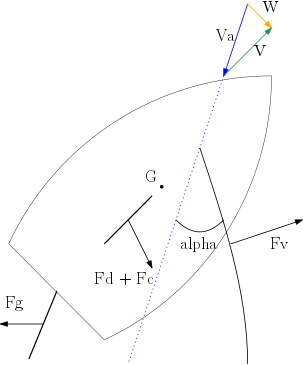
\includegraphics[scale=0.4]{trc.png} 
\end{figure}
\end{column}
\end{columns}
\end{frame}

\subsection{Commande par PID}

\begin{frame}
Régulateur PID agissant sur l'angle de barre $\beta$ en fonction de l'écart avec le cap $\delta$ :
\[ \beta = K( \delta + \frac{1}{\tau_{d}} \frac{d \delta}{dt} + \frac{1}{\tau_{i}} \int_{0}^{t} \delta (t)dt ) \]
L'écart avec le cap peut être remplacé par l'écart avec le vent au près.
\end{frame}

\begin{frame}\frametitle{Methode du régleur}
\begin{figure}
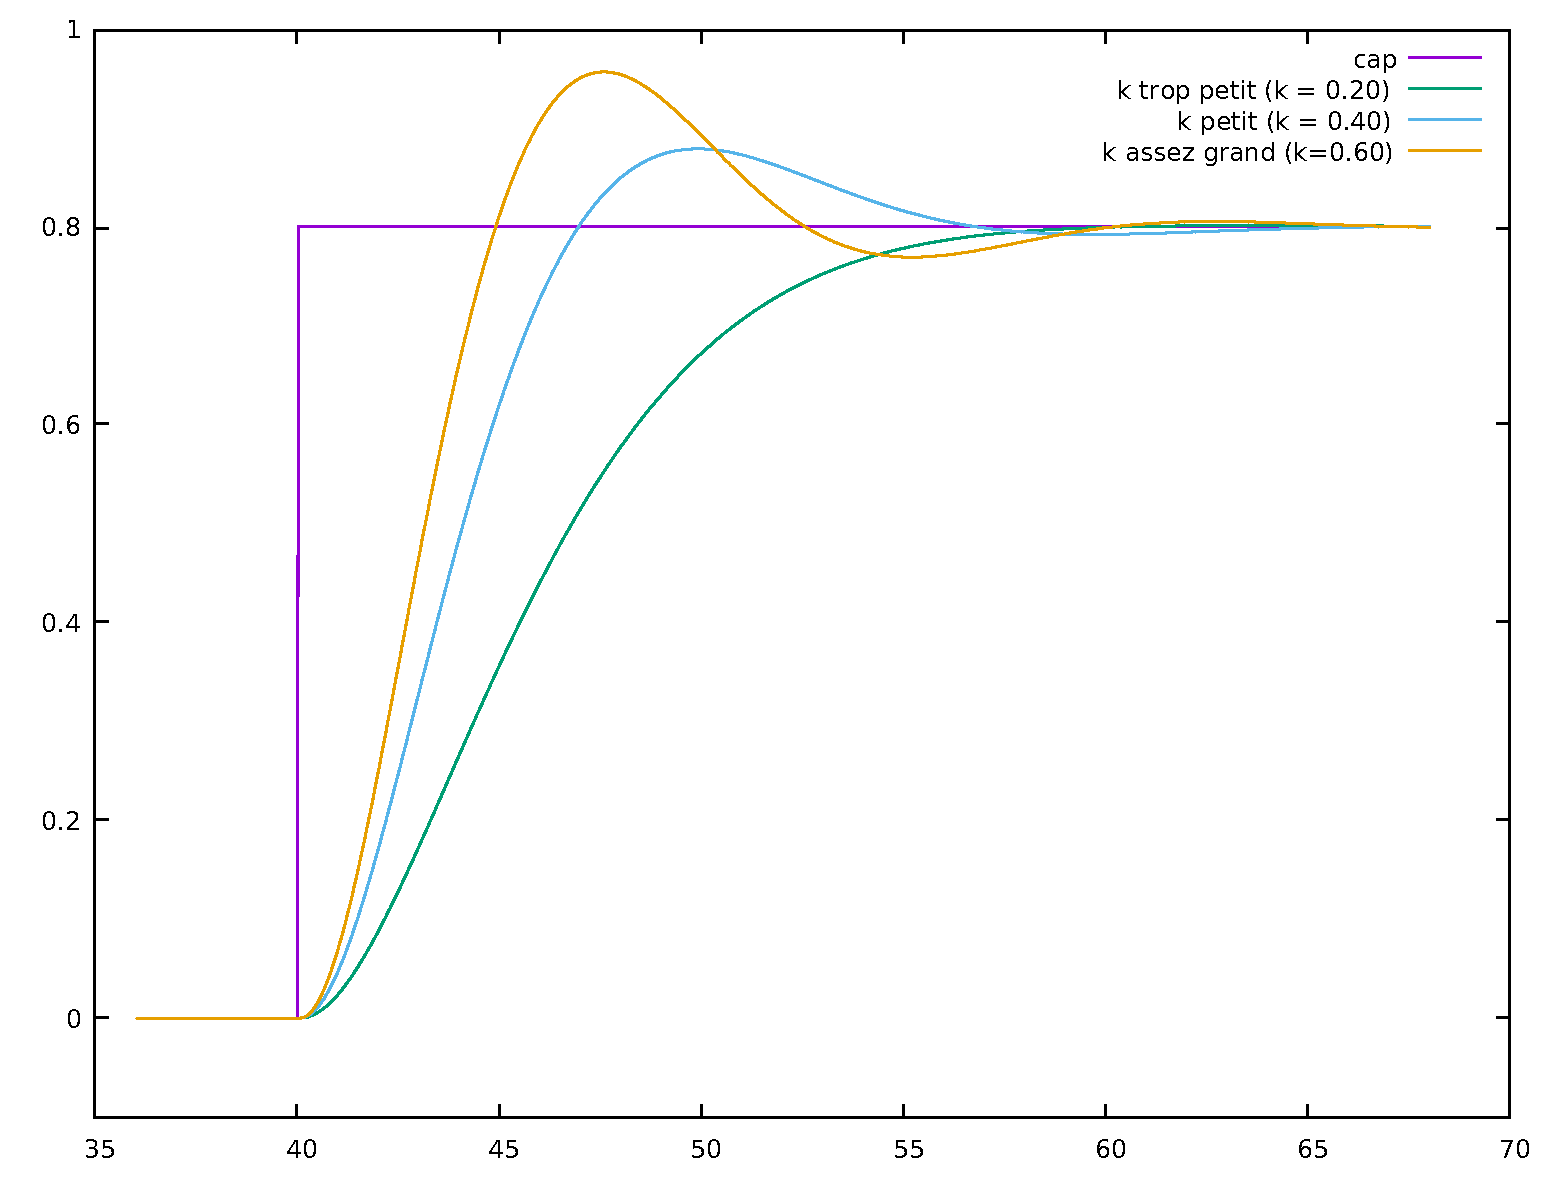
\includegraphics[scale=0.28]{courbesk.pdf} 
\caption{Réglage du gain K}
\end{figure}
\end{frame}

\begin{frame}\frametitle{Methode du régleur}
\begin{figure}
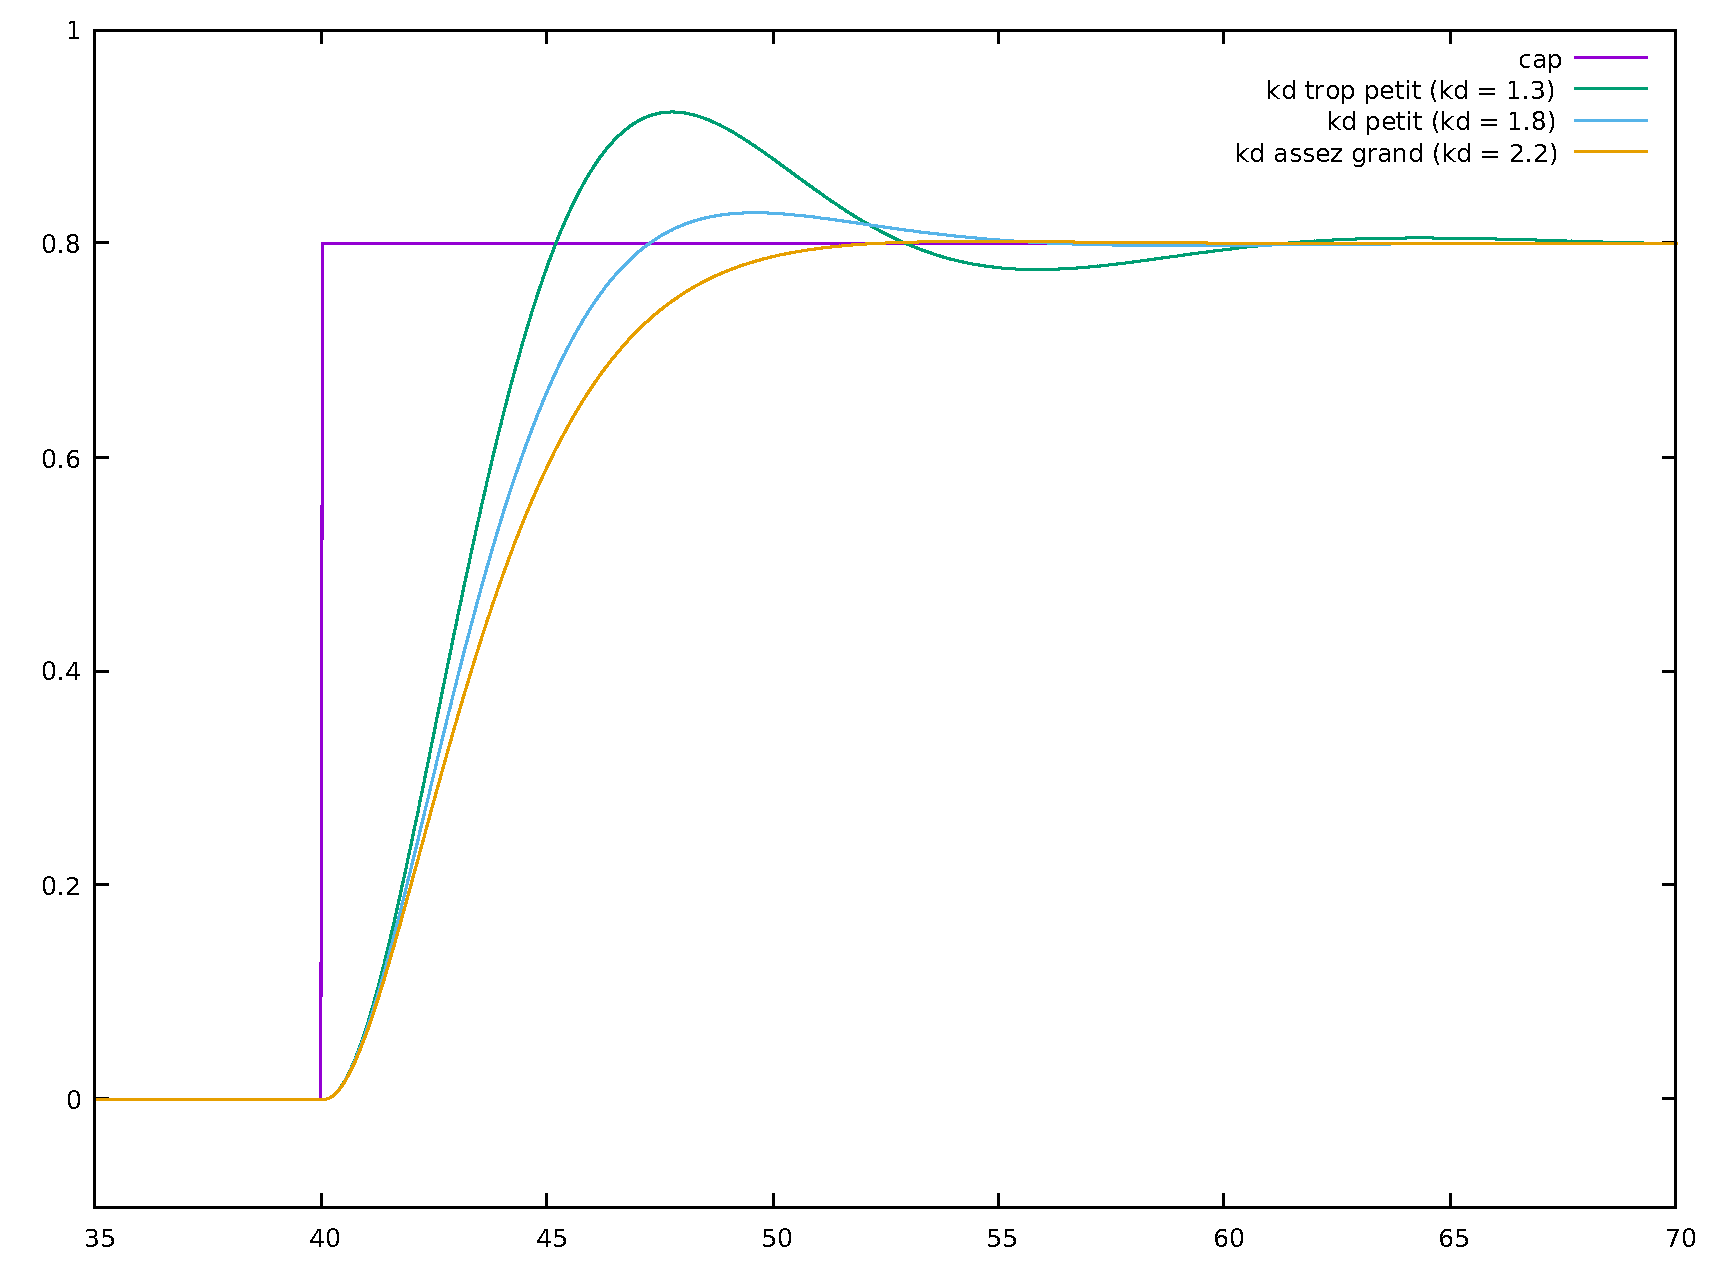
\includegraphics[scale=0.28]{courbeskd.pdf} 
\caption{Réglage de Kd}
\end{figure}
\end{frame}


\begin{frame}\frametitle{Affichage}
\begin{figure}
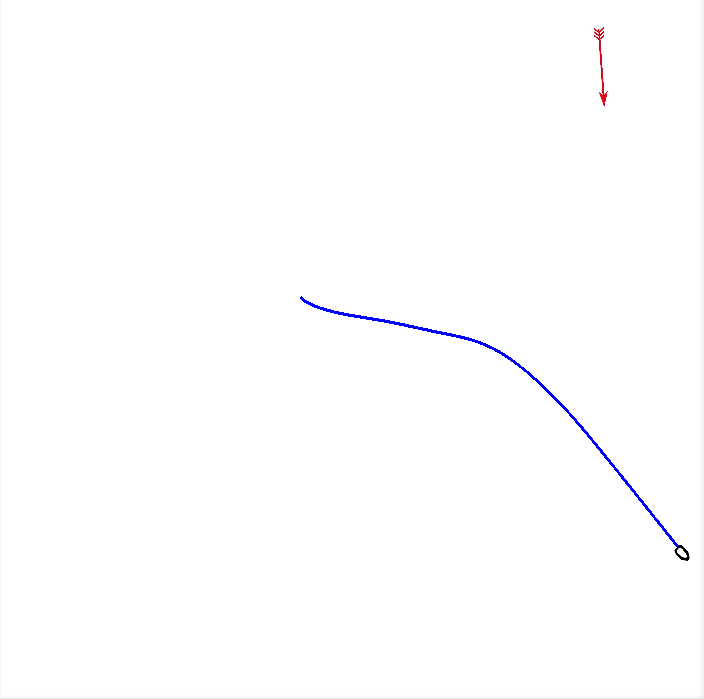
\includegraphics[scale=0.3]{Screenshot.png} 
\caption{Simulation du voilier}
\end{figure}
\end{frame}

\section{Pilotage avec un réseau de Petri}

\subsection{Rôle et définition }

\begin{frame}\frametitle{III Pilotage avec un  réseau de Petri: Rôle et définition}
\begin{block}{Rôle}
Le Réseau de Petri (RdP) est chargé de choisir la meilleure stratégie (relance, barre en mode cap ou vent) de pilotage en fonction des événements discrets qui pertubent le pilotage du voilier (rafale, molle, changement de direction du vent).
\end{block}
\begin{block}{Définition}
Un RdP est 5-tuplet $ R = (P, T, post, pre, \tau) $ avec:
\begin{itemize}
\item $P$ un ensemble non-vide fini de places
\item $Pre : P \times T \rightarrow \mathbb{R}$ une application d'incidence avant
\item $Post : P \times T \rightarrow \mathbb{R}$ une application d'incidence arriere
\item $\tau \in \mathbb{N}^{P}$ est la temporisation associée aux places
\end{itemize}
Le marquage $M$ d'un RdP est une application $M : P \rightarrow \mathbb{N}$
\end{block}
\end{frame}

\subsection{Illustration du RdP}

\begin{frame}[plain]
\begin{figure}
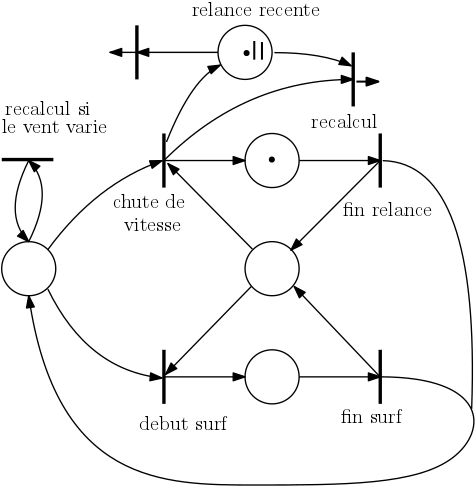
\includegraphics[scale=0.5]{rdp2.png} 
\caption{Illustration du RdP utilisé}
\end{figure}
\end{frame}

\subsection{Optimisation du pilotage}

\begin{frame}
\begin{figure}
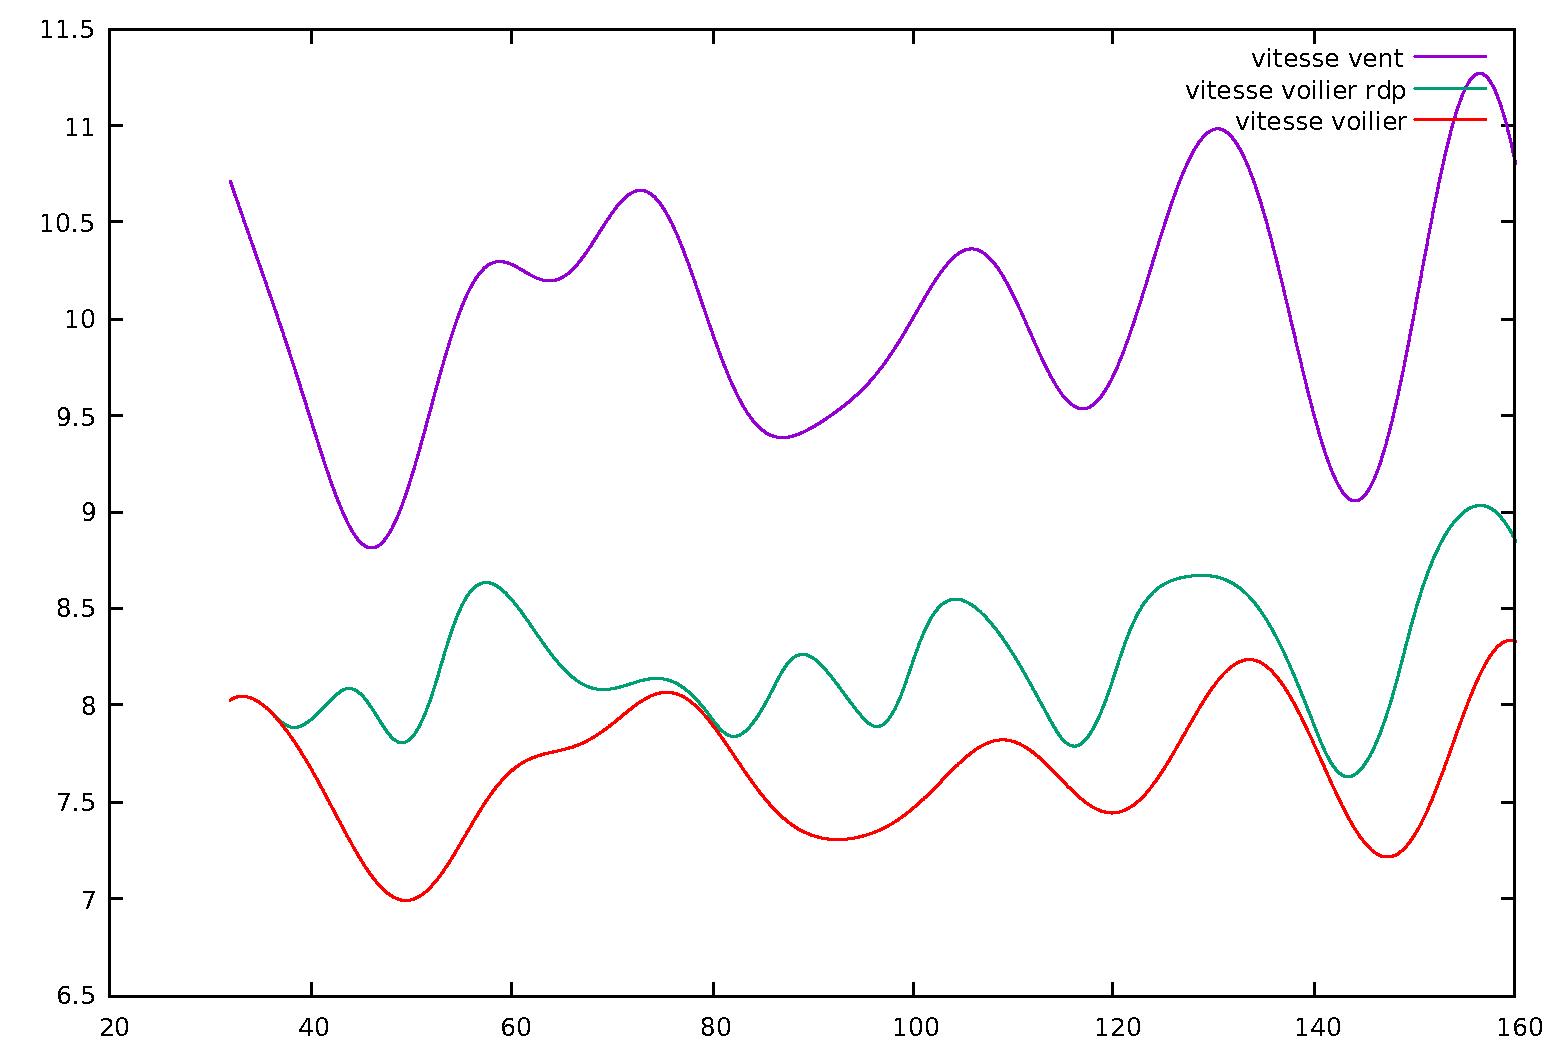
\includegraphics[scale=0.4]{vitesses.pdf} 
\caption{Comparaison des vitesses}
\end{figure}
\end{frame}

\begin{frame}[plain]
\begin{figure}
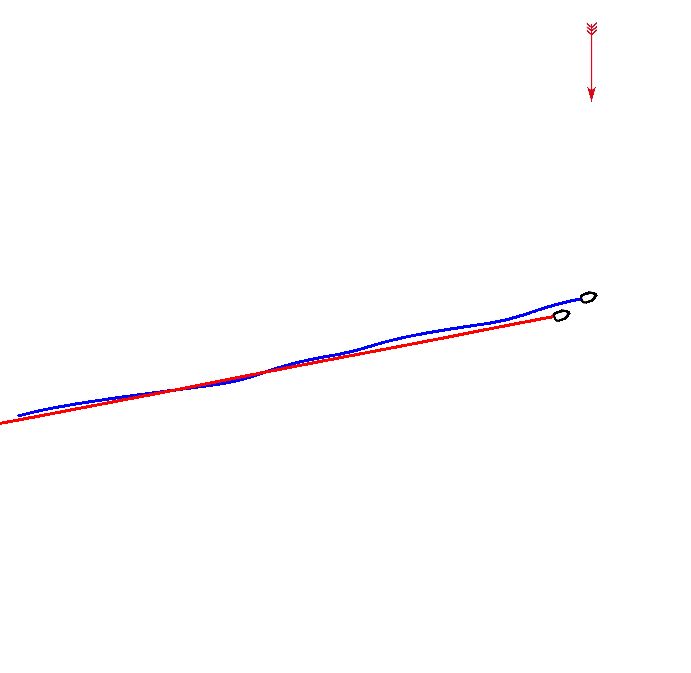
\includegraphics[scale=0.35]{Screenshot3.png} 
\caption{Trajectoire du voilier avec et sans RdP}
\end{figure}
\end{frame}



\begin{frame}[plain]\frametitle{Algorithme de Simulation}
\begin{figure}
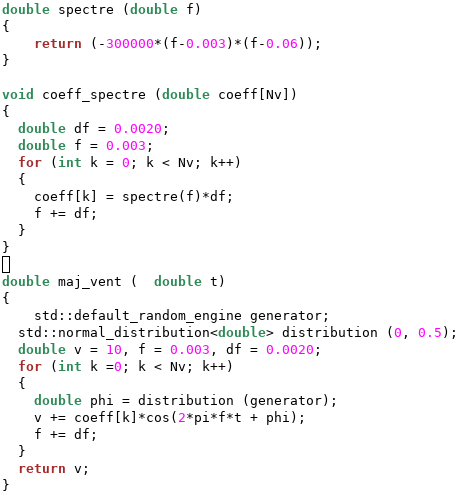
\includegraphics[scale=0.35]{sim1.png} 
\end{figure}
\end{frame}

\begin{frame}[plain]
\begin{figure}
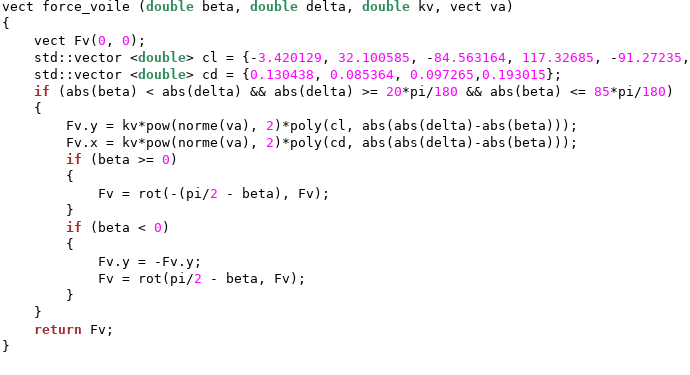
\includegraphics[scale=0.35]{sim2.png} 
\end{figure}
\end{frame}

\begin{frame}[plain]
\begin{figure}
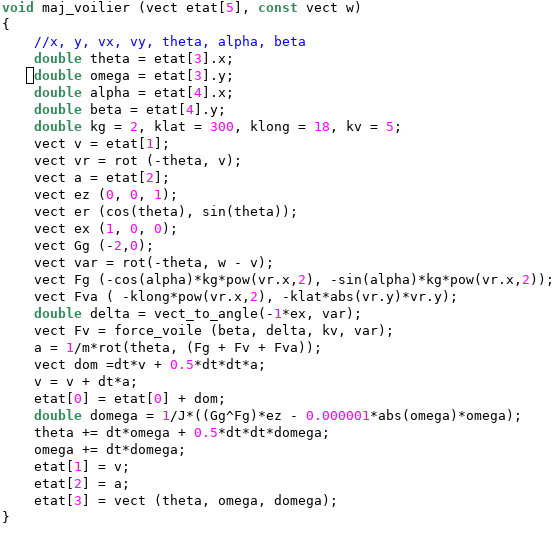
\includegraphics[scale=0.35]{sim3.png} 
\end{figure}
\end{frame}

\begin{frame}[plain]
\begin{figure}
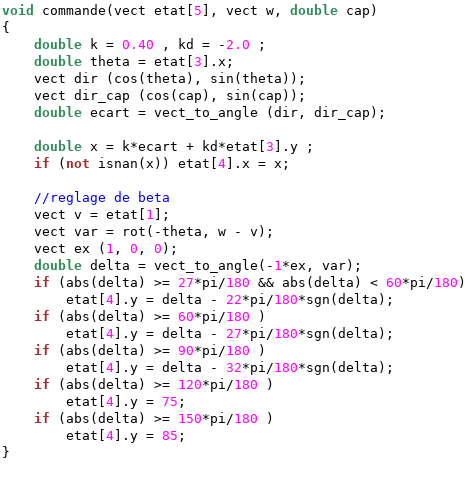
\includegraphics[scale=0.35]{sim4.png} 
\end{figure}
\end{frame}

\begin{frame}[plain]
\begin{figure}
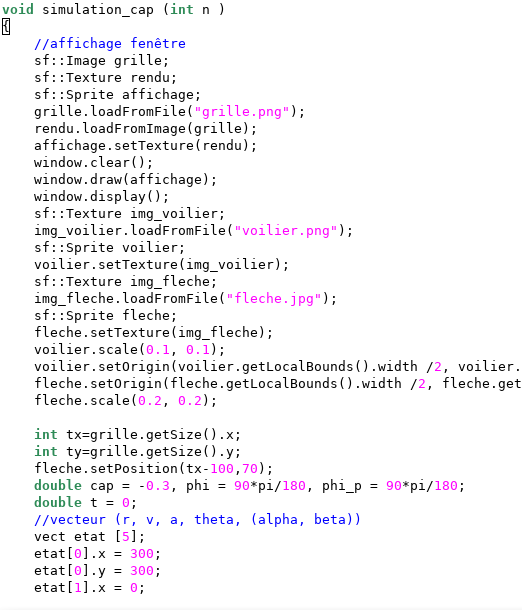
\includegraphics[scale=0.35]{sim5.png} 
\end{figure}
\end{frame}

\begin{frame}[plain]
\begin{figure}
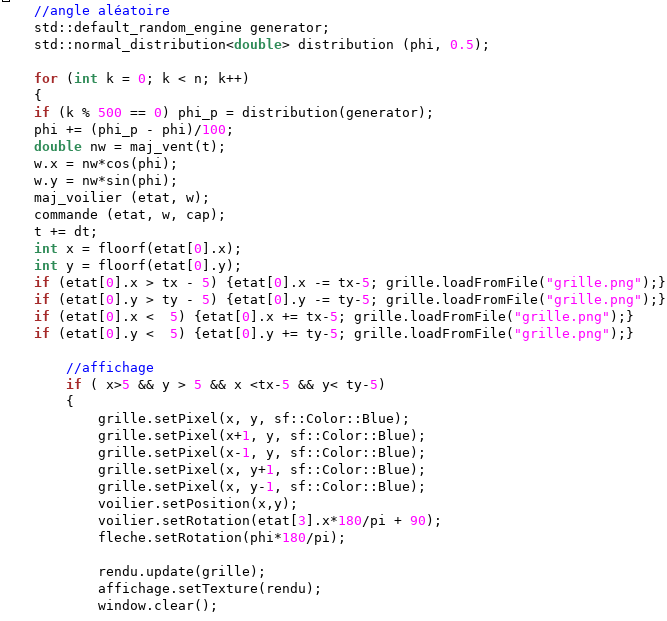
\includegraphics[scale=0.35]{sim6.png} 
\end{figure}
\end{frame}

\begin{frame}[plain]\frametitle{Algorithme de Dijkstra}
\begin{figure}
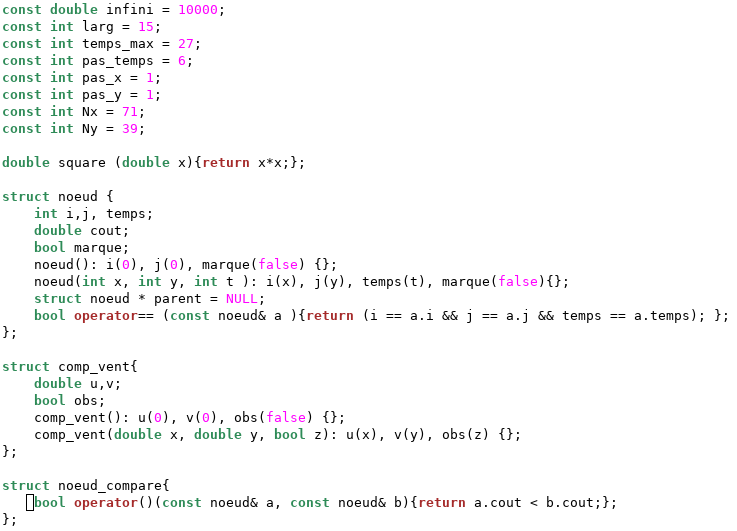
\includegraphics[scale=0.35]{dij1.png} 
\end{figure}
\end{frame}

\begin{frame}[plain]
\begin{figure}
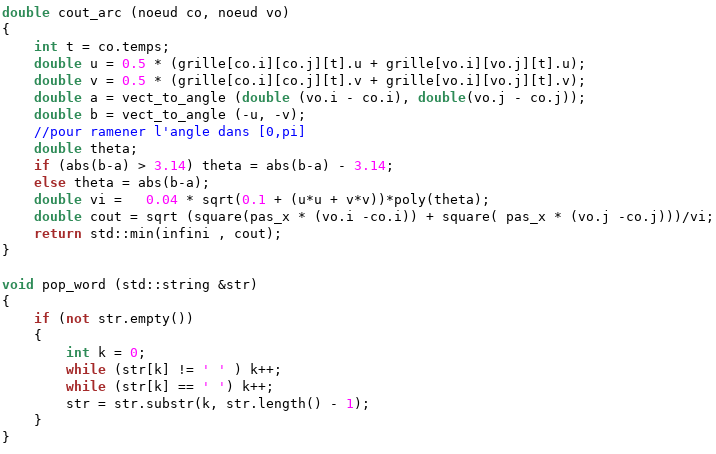
\includegraphics[scale=0.35]{dij2.png} 
\end{figure}
\end{frame}

\begin{frame}[plain]
\begin{figure}
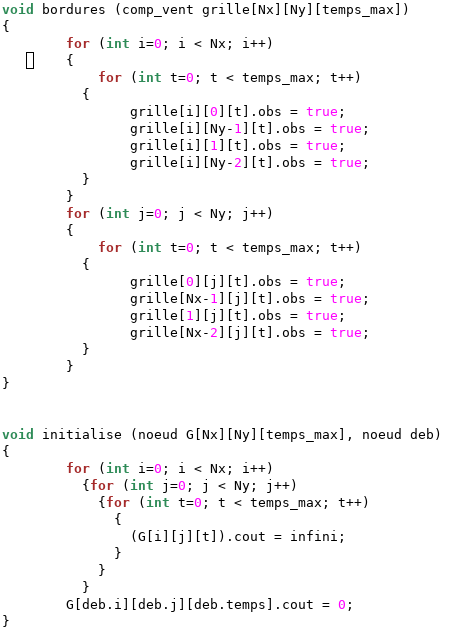
\includegraphics[scale=0.35]{dij3.png} 
\end{figure}
\end{frame}

\begin{frame}[plain]
\begin{figure}
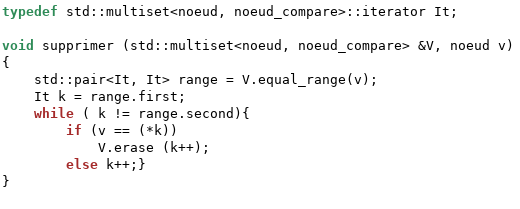
\includegraphics[scale=0.35]{dij4.png} 
\end{figure}
\end{frame}

\begin{frame}[plain]
\begin{figure}
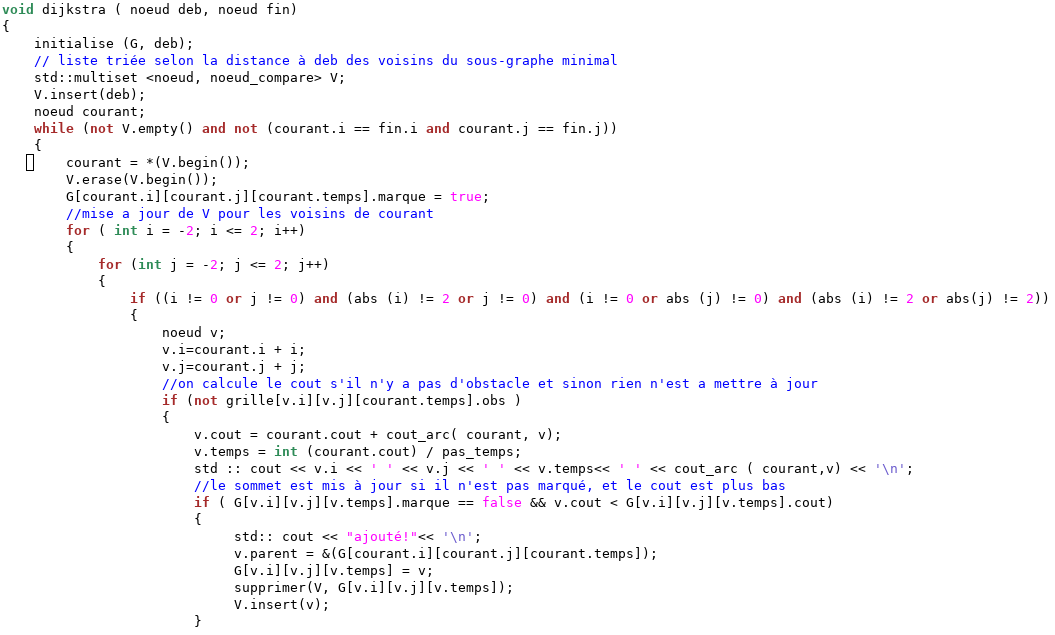
\includegraphics[scale=0.35]{dij5.png} 
\end{figure}
\end{frame}

\end{document}